\documentclass{standalone}
\usepackage{tikz}
\usetikzlibrary{patterns, positioning}


\begin{document}
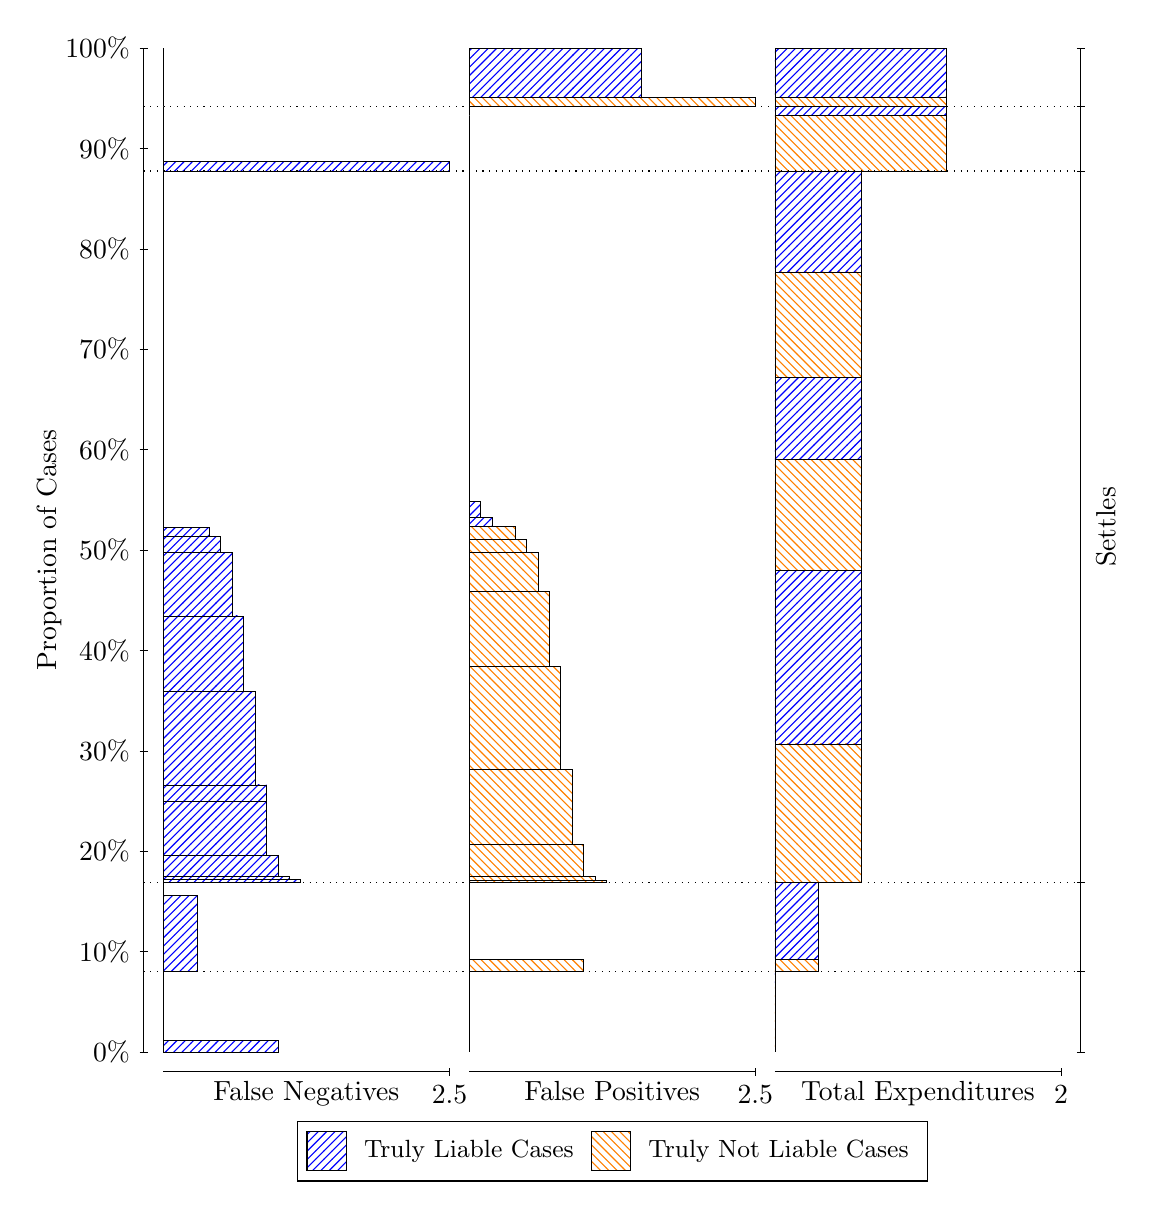
\begin{tikzpicture}
\draw[black, very thin] (1.5,1.75) -- (1.5,14.5);
\node[rotate=90, text=black, anchor=center] at (0.3, 8.125) {Proportion of Cases};
\draw[black, very thin] (1.45,1.75) -- (1.55,1.75);
\node[text=black, anchor=east] at (1.45, 1.75) {0\%};
\draw[black, very thin] (1.45,3.025) -- (1.55,3.025);
\node[text=black, anchor=east] at (1.45, 3.025) {10\%};
\draw[black, very thin] (1.45,4.3) -- (1.55,4.3);
\node[text=black, anchor=east] at (1.45, 4.3) {20\%};
\draw[black, very thin] (1.45,5.575) -- (1.55,5.575);
\node[text=black, anchor=east] at (1.45, 5.575) {30\%};
\draw[black, very thin] (1.45,6.85) -- (1.55,6.85);
\node[text=black, anchor=east] at (1.45, 6.85) {40\%};
\draw[black, very thin] (1.45,8.125) -- (1.55,8.125);
\node[text=black, anchor=east] at (1.45, 8.125) {50\%};
\draw[black, very thin] (1.45,9.4) -- (1.55,9.4);
\node[text=black, anchor=east] at (1.45, 9.4) {60\%};
\draw[black, very thin] (1.45,10.675) -- (1.55,10.675);
\node[text=black, anchor=east] at (1.45, 10.675) {70\%};
\draw[black, very thin] (1.45,11.95) -- (1.55,11.95);
\node[text=black, anchor=east] at (1.45, 11.95) {80\%};
\draw[black, very thin] (1.45,13.225) -- (1.55,13.225);
\node[text=black, anchor=east] at (1.45, 13.225) {90\%};
\draw[black, very thin] (1.45,14.5) -- (1.55,14.5);
\node[text=black, anchor=east] at (1.45, 14.5) {100\%};

\draw[black, very thin] (13.4,1.75) -- (13.4,14.5);
\draw[black, very thin] (13.35,1.75) -- (13.45,1.75);
\node[anchor=west] at (13.35, 1.75) {};
\draw[black, very thin] (13.35,2.769) -- (13.45,2.769);
\node[anchor=west] at (13.35, 2.769) {};
\draw[black, very thin] (13.35,3.8989) -- (13.45,3.8989);
\node[anchor=west] at (13.35, 3.8989) {};
\draw[black, very thin] (13.35,12.938) -- (13.45,12.938);
\node[anchor=west] at (13.35, 12.938) {};
\draw[black, very thin] (13.35,13.758) -- (13.45,13.758);
\node[anchor=west] at (13.35, 13.758) {};
\draw[black, very thin] (13.35,14.5) -- (13.45,14.5);
\node[anchor=west] at (13.35, 14.5) {};

\draw[black, very thin, pattern color=blue, pattern=north east lines] (1.75,1.75) rectangle (3.2033,1.893);
\draw[black, very thin, pattern color=orange, pattern=north west lines] (1.75,1.893) rectangle (1.75,2.769);
\draw[black, very thin, pattern color=blue, pattern=north east lines] (1.75,2.769) rectangle (2.186,3.7428);
\draw[black, very thin, pattern color=orange, pattern=north west lines] (1.75,3.7428) rectangle (1.75,3.8989);
\draw[black, very thin, pattern color=blue, pattern=north east lines] (1.75,3.8989) rectangle (3.494,3.9425);
\draw[black, very thin, pattern color=blue, pattern=north east lines] (1.75,3.9425) rectangle (3.3487,3.9848);
\draw[black, very thin, pattern color=blue, pattern=north east lines] (1.75,3.9848) rectangle (3.2033,4.2437);
\draw[black, very thin, pattern color=blue, pattern=north east lines] (1.75,4.2437) rectangle (3.058,4.9341);
\draw[black, very thin, pattern color=blue, pattern=north east lines] (1.75,4.9341) rectangle (3.058,5.1419);
\draw[black, very thin, pattern color=blue, pattern=north east lines] (1.75,5.1419) rectangle (2.9127,6.3317);
\draw[black, very thin, pattern color=blue, pattern=north east lines] (1.75,6.3317) rectangle (2.7673,7.2888);
\draw[black, very thin, pattern color=blue, pattern=north east lines] (1.75,7.2888) rectangle (2.622,8.0965);
\draw[black, very thin, pattern color=blue, pattern=north east lines] (1.75,8.0965) rectangle (2.4767,8.3002);
\draw[black, very thin, pattern color=blue, pattern=north east lines] (1.75,8.3002) rectangle (2.3313,8.4147);
\draw[black, very thin, pattern color=orange, pattern=north west lines] (1.75,8.4147) rectangle (1.75,12.938);
\draw[black, very thin, pattern color=blue, pattern=north east lines] (1.75,12.938) rectangle (5.3833,13.056);
\draw[black, very thin, pattern color=orange, pattern=north west lines] (1.75,13.056) rectangle (1.75,13.758);
\draw[black, very thin, pattern color=orange, pattern=north west lines] (1.75,13.758) rectangle (1.75,13.876);
\draw[black, very thin, pattern color=blue, pattern=north east lines] (1.75,13.876) rectangle (1.75,14.5);
\draw[black, very thin, pattern color=orange, pattern=north west lines] (5.6333,1.75) rectangle (5.6333,2.626);
\draw[black, very thin, pattern color=blue, pattern=north east lines] (5.6333,2.626) rectangle (5.6333,2.769);
\draw[black, very thin, pattern color=orange, pattern=north west lines] (5.6333,2.769) rectangle (7.0867,2.9252);
\draw[black, very thin, pattern color=blue, pattern=north east lines] (5.6333,2.9252) rectangle (5.6333,3.8989);
\draw[black, very thin, pattern color=orange, pattern=north west lines] (5.6333,3.8989) rectangle (7.3773,3.9324);
\draw[black, very thin, pattern color=orange, pattern=north west lines] (5.6333,3.9324) rectangle (7.232,3.9786);
\draw[black, very thin, pattern color=orange, pattern=north west lines] (5.6333,3.9786) rectangle (7.0867,4.3879);
\draw[black, very thin, pattern color=orange, pattern=north west lines] (5.6333,4.3879) rectangle (6.9413,5.3412);
\draw[black, very thin, pattern color=orange, pattern=north west lines] (5.6333,5.3412) rectangle (6.796,6.6506);
\draw[black, very thin, pattern color=orange, pattern=north west lines] (5.6333,6.6506) rectangle (6.6507,7.5953);
\draw[black, very thin, pattern color=orange, pattern=north west lines] (5.6333,7.5953) rectangle (6.5053,8.099);
\draw[black, very thin, pattern color=orange, pattern=north west lines] (5.6333,8.099) rectangle (6.36,8.2566);
\draw[black, very thin, pattern color=orange, pattern=north west lines] (5.6333,8.2566) rectangle (6.2147,8.4218);
\draw[black, very thin, pattern color=blue, pattern=north east lines] (5.6333,8.4218) rectangle (5.924,8.5363);
\draw[black, very thin, pattern color=blue, pattern=north east lines] (5.6333,8.5363) rectangle (5.7787,8.7401);
\draw[black, very thin, pattern color=blue, pattern=north east lines] (5.6333,8.7401) rectangle (5.6333,12.938);
\draw[black, very thin, pattern color=orange, pattern=north west lines] (5.6333,12.938) rectangle (5.6333,13.64);
\draw[black, very thin, pattern color=blue, pattern=north east lines] (5.6333,13.64) rectangle (5.6333,13.758);
\draw[black, very thin, pattern color=orange, pattern=north west lines] (5.6333,13.758) rectangle (9.2667,13.876);
\draw[black, very thin, pattern color=blue, pattern=north east lines] (5.6333,13.876) rectangle (7.8133,14.5);
\draw[black, very thin, pattern color=orange, pattern=north west lines] (9.5167,1.75) rectangle (9.5167,2.626);
\draw[black, very thin, pattern color=blue, pattern=north east lines] (9.5167,2.626) rectangle (9.5167,2.769);
\draw[black, very thin, pattern color=orange, pattern=north west lines] (9.5167,2.769) rectangle (10.062,2.9252);
\draw[black, very thin, pattern color=blue, pattern=north east lines] (9.5167,2.9252) rectangle (10.062,3.8989);
\draw[black, very thin, pattern color=orange, pattern=north west lines] (9.5167,3.8989) rectangle (10.607,5.6639);
\draw[black, very thin, pattern color=blue, pattern=north east lines] (9.5167,5.6639) rectangle (10.607,7.865);
\draw[black, very thin, pattern color=orange, pattern=north west lines] (9.5167,7.865) rectangle (10.607,9.2793);
\draw[black, very thin, pattern color=blue, pattern=north east lines] (9.5167,9.2793) rectangle (10.607,10.314);
\draw[black, very thin, pattern color=orange, pattern=north west lines] (9.5167,10.314) rectangle (10.607,11.658);
\draw[black, very thin, pattern color=blue, pattern=north east lines] (9.5167,11.658) rectangle (10.607,12.938);
\draw[black, very thin, pattern color=orange, pattern=north west lines] (9.5167,12.938) rectangle (11.697,13.64);
\draw[black, very thin, pattern color=blue, pattern=north east lines] (9.5167,13.64) rectangle (11.697,13.758);
\draw[black, very thin, pattern color=orange, pattern=north west lines] (9.5167,13.758) rectangle (11.697,13.876);
\draw[black, very thin, pattern color=blue, pattern=north east lines] (9.5167,13.876) rectangle (11.697,14.5);
\draw[black, dotted] (1.5,2.769) -- (13.4,2.769);
\draw[black, dotted] (1.5,3.8989) -- (13.4,3.8989);
\draw[black, dotted] (1.5,12.938) -- (13.4,12.938);
\draw[black, dotted] (1.5,13.758) -- (13.4,13.758);
\draw[black, very thin] (1.75,1.5) -- (5.3833,1.5);
\node[text=black, anchor=north] at (3.5667, 1.5) {False Negatives};
\draw[black, very thin] (5.3833,1.45) -- (5.3833,1.55);
\node[text=black, anchor=north] at (5.3833, 1.45) {2.5};

\draw[black, very thin] (5.6333,1.5) -- (9.2667,1.5);
\node[text=black, anchor=north] at (7.45, 1.5) {False Positives};
\draw[black, very thin] (9.2667,1.45) -- (9.2667,1.55);
\node[text=black, anchor=north] at (9.2667, 1.45) {2.5};

\draw[black, very thin] (9.5167,1.5) -- (13.15,1.5);
\node[text=black, anchor=north] at (11.333, 1.5) {Total Expenditures};
\draw[black, very thin] (13.15,1.45) -- (13.15,1.55);
\node[text=black, anchor=north] at (13.15, 1.45) {2};



\node[text=black, centered, rotate=90] at (13.72, 8.4183) {Settles};



\draw (7.449999999999999,1.5) node[draw=none] (baseCoordinate) {};
\begin{scope}[align=center]
        \matrix[scale=0.5, draw=black, below=0.5cm of baseCoordinate, nodes={draw}, column sep=0.1cm]{
            \node[rectangle, draw, minimum width=0.5cm, minimum height=0.5cm, pattern color=blue, pattern=north east lines] {}; &
            \node[draw=none, font=\small, text=black] (B) {Truly Liable Cases}; &
            \node[rectangle, draw, minimum width=0.5cm, minimum height=0.5cm, pattern color=orange, pattern=north west lines] {}; &
            \node[draw=none, font=\small, text=black] (B) {Truly Not Liable Cases}; \\
            };
\end{scope}

\end{tikzpicture}
\end{document}